% Technical report template (acmart sigconf). Numbers written as a name between double at-signs are filled
% by tools/fill_report.py from results/final_results.json so that text, tables and figures stay consistent.
\documentclass[sigconf]{acmart}
\settopmatter{printacmref=false}
\renewcommand\footnotetextcopyrightpermission[1]{}
\setcopyright{none}
\acmConference[]{}{}{}
\acmYear{2026}
\acmISBN{}
\acmDOI{}
\pagestyle{plain}
\usepackage{booktabs}
\usepackage{graphicx}
\usepackage{amsmath}
\emergencystretch=1.5em

\begin{document}

\title{Solar Filament Instance Segmentation with Test-Time Voting}
\subtitle{A Solution to the Solar Filament Segmentation Challenge 2026} % DO NOT CHANGE

\author{NIklitaCheporev}
\affiliation{%
  \institution{Independent}
  \country{}
}

\begin{abstract}
This report describes our solution to the Solar Filament Segmentation Challenge 2026, a Kaggle competition on automatic segmentation of solar filaments in GONG H-$\alpha$ observations.
We train YOLO11s-seg instance detectors on the provided annotations only and combine 6 detectors and 8 dihedral test-time views by instance-level voting, followed by a $3\times3$ erosion and largest-component filtering.
On an observation-grouped holdout the pipeline reaches a Panoptic Quality of 0.425 (95\% CI [0.404, 0.444]), above the 0.340 agreement between independent experts.
We report observation-level uncertainty, agreement among independent annotations and the effect of the main pipeline stages.
\end{abstract}

\maketitle

\section{Introduction}
This report goes over the details of our submitted solution to the Solar Filament Segmentation Challenge 2026~\cite{challenge}. The challenge, launched on July 10, 2026, is organized by the Earth-Space AI Research (ESAIR) Lab\footnote{www.esairlab.com/}. This challenge utilizes the MAGFiLO dataset for evaluation of the segmentation algorithms~\cite{magfilo}.
We fine-tune COCO-initialized detectors on the provided training images and annotations. Each prediction uses the pixels of a single provided H-$\alpha$ image. We compare changes using paired bootstrap intervals over physical observations.

\section{Methodology}
\paragraph{Data and splits.}
The training set has 707 physical observations with 1\,154 independent annotator copies and 8\,199 filament polygons. A copy is one annotator's labelling of an image; the same JPEG therefore appears up to three times with different labels. Splitting by image id would leak the image between folds, so all splits are by physical observation and stratified by observatory: 566 observations for fitting and 141 (229 copies) as a holdout that is never used for training. Five observation-grouped folds of the fitting part provide out-of-fold predictions and the ensemble members.

\paragraph{Detector.}
We use YOLO11s-seg~\cite{ultralytics} initialised from COCO weights. Each annotator copy is a separate training example, so the network learns the \emph{typical} annotator. Stage~1 trains for 40 epochs at 1024\,px (mosaic, scale and colour augmentation); stage~2 fine-tunes at the native 2048\,px for 5 (first detector) or 6 (fold detectors) epochs (AdamW, learning rate $10^{-4}$, no mosaic). The fold detectors use fixed epoch counts and their last checkpoints, so no checkpoint is selected on held-out data; the first detector starts stage~2 from the validation-best epoch of its stage-1 run (epoch 39 of 40, 0.003 mask mAP$_{50\text{--}95}$ above the last epoch).

\paragraph{Inference pipeline (Fig.~\ref{fig:pipeline}).}
\begin{enumerate}\itemsep0pt
\item Every detector is applied to the 8 dihedral views of the image; masks are mapped back to the original frame.
\item Instances of all (detector, view) sources are clustered by IoU\,$>$\,0.3 with at most one member per source. The fused mask is the pixel vote of the members (at least half), its score the sum of member confidences divided by the number of sources.
\item Contested pixels go to the higher score, instances with a score below 0.18 are dropped.
\item Each mask is eroded with a $3\times3$ elliptical kernel. The detector predicts masks at quarter resolution and its outlines are systematically wider than the annotators' polygons; the erosion is the single most important post-processing step (+0.023 PQ).
\item Only the largest connected component of each mask is kept, so one detection is one filament piece.
\end{enumerate}
The repository\footnote{\url{https://github.com/gtrg55/filament-segmentation-2026}} contains the weights and a demo notebook for reproducing the predictions.

\begin{figure}[t]
\centering
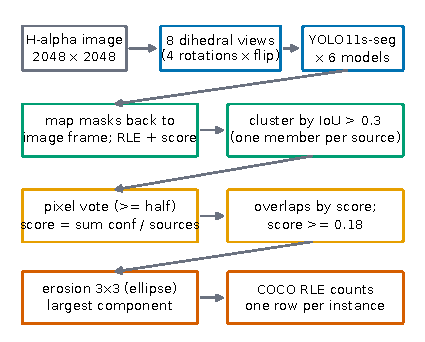
\includegraphics[width=0.92\columnwidth]{fig_pipeline.pdf}
\caption{Inference pipeline: dihedral views of one or more detectors, instance voting, overlap resolution, erosion and RLE export.}
\label{fig:pipeline}
\end{figure}

\paragraph{Alternatives evaluated.}
Paired comparisons covered other inference scales, softer box NMS, mask filtering and a ResNet34 U-Net. We also trained two filters on out-of-fold weak detections. A feature-based scorer and an image-crop classifier gave $\Delta$PQ of $-0.0010$ and $-0.0007$ against the frozen ensemble. Both 95\% intervals include zero.

\section{Evaluation}
\paragraph{Protocol.}
We reproduce the organizers' self-evaluation: every annotator copy is scored against the prediction of its observation, a pair with IoU\,$>$\,0.5 is a true positive, and Panoptic Quality~\cite{pq}, PQ\,=\,$\sum \mathrm{IoU}_{TP}/(|TP|+\tfrac12|FP|+\tfrac12|FN|)$, is pooled over copies. We also report the mean Dice of the union masks, the mean IoU and Dice of overlapping pairs and the rates of one-to-many (a ground-truth filament overlapped by $\ge2$ predictions) and many-to-one relations. Uncertainty is a bootstrap over observations (4000 draws); every change is compared with its parent by a \emph{paired} bootstrap on the same resamples. We chose the score threshold, erosion and largest-component step on out-of-fold predictions from the fitting split. The holdout was used for ensemble comparisons and the first detector's stage-1 checkpoint. Its repeated use limits how directly these intervals generalize to new observations.

\paragraph{Expert agreement.}
Scoring each annotator against the other annotators of the same image gives PQ 0.340 across 296 observations with two or three copies. The mean IoU among matched masks is 0.634. On observations with three copies, consensus masks from two annotators score 0.31--0.34 against the third across the rules tested. These scores describe variability across independent annotations.

\paragraph{Results.}
Table~\ref{tab:results} lists the holdout PQ of every pipeline stage with the paired gain over the previous stage; Fig.~\ref{fig:results} shows the same intervals next to the expert-agreement level.
\begin{table}[t]
\centering\small\setlength{\tabcolsep}{1.5pt}
\caption{Pipeline stages on the holdout (141 observations, 229 annotator copies). PQ with 95\% bootstrap interval; $\Delta$PQ is the paired gain over the previous row; Dice is the mean Dice of the union masks.}
\label{tab:results}
\begin{tabular}{@{}lccc@{}}
\toprule
 Stage & PQ [95\% CI] & $\Delta$PQ [95\% CI] & Dice \\
\midrule
1 detector, 1 view & 0.382 [0.361, 0.403] & -- & 0.614 \\
+ 3x3 erosion & 0.405 [0.384, 0.426] & +0.023 [+0.016, +0.031] & 0.621 \\
+ 8 dihedral views & 0.423 [0.402, 0.443] & +0.019 [+0.008, +0.029] & 0.632 \\
+ 5 more detectors & 0.425 [0.405, 0.444] & +0.002 [$-$0.005, +0.009] & 0.656 \\
\textbf{+ largest component} & \textbf{0.425} [0.404, 0.444] & $-$0.001 [$-$0.004, +0.003] & 0.649 \\
\bottomrule
\end{tabular}
\end{table}

\begin{figure*}[t]
\centering
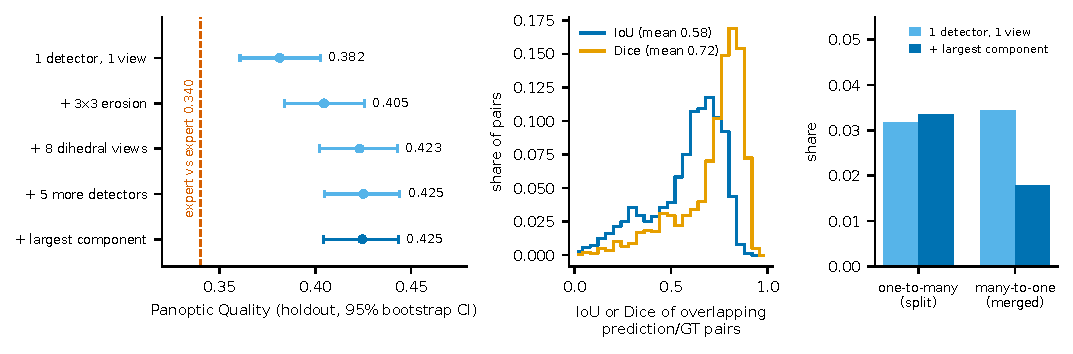
\includegraphics[width=\textwidth]{fig_results.pdf}
\caption{Left: PQ with 95\% bootstrap intervals for the pipeline stages and the expert-agreement level. Middle and right: IoU and Dice of overlapping prediction/ground-truth pairs and one-to-many / many-to-one rates of the final pipeline.}
\label{fig:results}
\end{figure*}

\paragraph{Test-time compute.} Detector ensembling and dihedral views are largely redundant (Table~\ref{tab:variants}): six detectors on a single view gain 0.010 PQ over one detector, eight views of one detector 0.019, and both together only 0.021. Halving the views to four costs nothing measurable (0.426--0.427 PQ against 0.425); we keep all 48 sources because the full vote has the best Dice (0.656), and inference is cheap (about 14\,s per image on an M4 Max).

\begin{table}[t]
\centering\small\setlength{\tabcolsep}{1.5pt}
\caption{Inference cost versus quality on the holdout. Sources = detectors $\times$ views; the score threshold is optimised per row, $\Delta$PQ is the paired gain over one detector with eight views; the largest-component step is not applied.}
\label{tab:variants}
\begin{tabular}{@{}lrccc@{}}
\toprule
 Configuration & Sources & PQ & $\Delta$PQ [95\% CI] & Dice \\
\midrule
1 detector, 1 view & 1 & 0.405 & $-$0.019 [$-$0.029, $-$0.008] & 0.621 \\
6 detectors, 1 view & 6 & 0.415 & $-$0.009 [$-$0.017, $-$0.000] & 0.639 \\
1 detector, 8 views & 8 & 0.423 & -- & 0.632 \\
6 detectors, 4 rotations & 24 & 0.427 & +0.004 [$-$0.004, +0.011] & 0.634 \\
6 detectors, 4 views (2 flips) & 24 & 0.426 & +0.003 [$-$0.004, +0.011] & 0.651 \\
5 fold detectors, 8 views & 40 & 0.425 & +0.002 [$-$0.005, +0.009] & 0.654 \\
6 detectors, 8 views & 48 & 0.425 & +0.002 [$-$0.005, +0.009] & 0.656 \\
\bottomrule
\end{tabular}
\end{table}

\paragraph{Morphology of the predicted masks.}
Annotators outline 7.0 filaments per image (median area 1296\,px$^2$, median thickness 16.1\,px, solidity 0.58, elongation 3.6); the final pipeline predicts 7.0 instances per image (median area 1342\,px$^2$, thickness 17.4\,px, solidity 0.66, elongation 3.9), i.e. smoother and more compact outlines than hand-drawn polygons and 1.2\,px thicker at the median. Annotated instances are almost always one connected component (99.8\%); the largest-component step makes every predicted instance one as well. Instance relations quantify the structural errors: 3.4\% of the annotated filaments are overlapped by two or more predictions (one-to-many; 3.2\% for a single view) and 1.8\% of the predictions overlap two or more annotated filaments (many-to-one; 3.4\% for a single view). Overlapping pairs have a mean IoU of 0.58 and a mean Dice of 0.72 (Fig.~\ref{fig:results}); Fig.~\ref{fig:examples} shows holdout crops at fixed percentiles of the per-observation PQ.

\begin{figure*}[t]
\centering
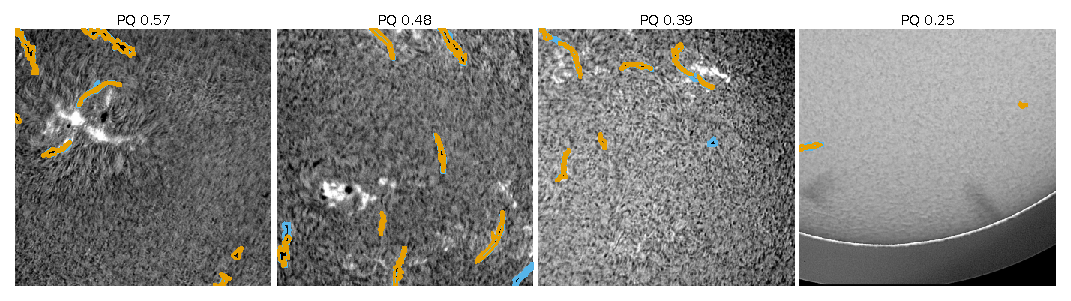
\includegraphics[width=\textwidth]{fig_examples.pdf}
\caption{Holdout crops (768$\times$768\,px of 2048) of observations at the 90th, 65th, 35th and 10th percentile of per-observation PQ (not hand-picked): outlines of one annotator copy (orange) and of the predicted instances (blue).}
\label{fig:examples}
\end{figure*}

\paragraph{Where the errors are.}
Recall depends on size (Fig.~\ref{fig:errors}): 42.8\% of the smallest quintile of annotated filaments (below 615\,px$^2$) are matched, 64.8\%--77.7\% of the middle quintiles, and 57.8\% of the largest (above 2975\,px$^2$), where an IoU above 0.5 requires agreeing on the whole extent of a long structure. Precision is 72.4\%--74.9\% except for the smallest predicted quintile (64.3\%). PQ by observatory ranges from 0.395 (Bh, 24 observations) to 0.474 (Uh, 20). Each estimate uses 20--25 observations.

\begin{figure}[t]
\centering
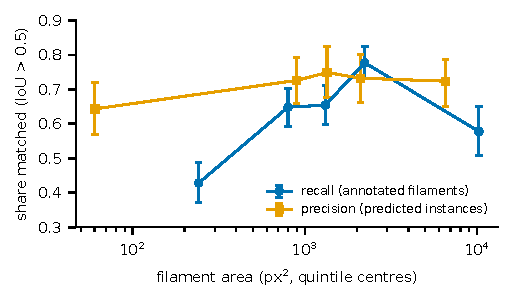
\includegraphics[width=\columnwidth]{fig_errors.pdf}
\caption{Share of annotated filaments that are matched (recall) and of predicted instances that match an annotator (precision), by area quintile on the holdout; bars are 95\% observation-level bootstrap intervals.}
\label{fig:errors}
\end{figure}

\paragraph{Leaderboard calibration.}
Earlier single-detector submissions had holdout PQ and public score pairs (0.289$\to$0.24, 0.384$\to$0.34, 0.405$\to$0.36). The gaps ranged from 0.044 to 0.049 across these 3 submissions. The final pipeline scored 0.37 publicly and 0.425 on the holdout. The public forecast was 0.38 and the holdout-to-public gap was 0.055. Kaggle displays the public score to two decimal places. A split-half check estimated 0.002 PQ of selection optimism for the tested threshold and erosion grid.
\paragraph{Second submission.} We refit two detectors on all 707 observations and applied the same post-processing. The second submission scored 0.37 publicly. Its predictions and those of the first submission agreed at PQ 0.905.

\paragraph{Earlier control submissions.} Early in the competition we also submitted outputs derived from public notebooks as attributed controls (public scores between 0.34 and 0.56). They are not part of this solution; the two final submissions come only from the detectors described here.

\paragraph{Strengths, weaknesses, improvements.}
\emph{Strengths.} The solution is a single public architecture trained on the provided labels, evaluated with an observation-grouped protocol; every claimed gain has a paired interval. Erosion, voting over views and voting over detectors turn near-misses into matches and remove false alarms (901 $\to$ 994 true positives, 583 $\to$ 567 false positives). Individually, the five fold detectors (trained on 80\% of the fit observations) reach 0.411--0.422 PQ with eight views (mean 0.417) against 0.423 for the first detector; the six-detector vote adds +0.002 PQ (paired 95\% CI [$-$0.005, +0.009]) and +0.024 Dice. Matched filaments agree with the annotator slightly better than experts agree with each other (IoU 0.68 vs 0.63). \emph{Weaknesses.} 19.8\% of annotated filaments have zero overlap with every prediction. Recognition quality is 0.63 for the detector and 0.54 between annotators. The smallest area quintile has the lowest recall. \emph{Improvements.} Further experiments can target the extent of long masks and the detection of small filaments.

\begin{acks}
The organization of the Filament Segmentation Challenge 2026 is partially supported by the U.S. National Science Foundation (NSF) under Grant No. 2209912 and 2433781, directorate for Computer and Information Science and Engineering (CSE), and Office of Advanced Cyberinfrastructure (OAC), and Grant No. 2511630, AST Division Of Astronomical Sciences and MPS Directorate for Mathematical and Physical Sciences.

The Filament Segmentation Challenge 2026 is sponsored by the U.S. National Science Foundation (NSF) National Solar Observatory (NSO).

This work utilizes GONG data obtained by the NSO Integrated Synoptic Program, managed by the National Solar Observatory, which is operated by the Association of Universities for Research in Astronomy (AURA), Inc. under a cooperative agreement with the National Science Foundation and with contribution from the National Oceanic and Atmospheric Administration. The GONG network of instruments is hosted by the Big Bear Solar Observatory, High Altitude Observatory, Learmonth Solar Observatory, Udaipur Solar Observatory, Instituto de Astrof\'isica de Canarias, and Cerro Tololo Interamerican Observatory.
\end{acks}

\bibliographystyle{ACM-Reference-Format}
\bibliography{main}

\end{document}
